\documentclass{article}
\usepackage{graphicx}
\usepackage{geometry}
\usepackage[MeX]{polski}
\usepackage[polish]{babel}
% Make header with name and date etc.
\usepackage{fancyhdr}
\lhead{Zuzanna Cienka\\nr albumu 148201}
\rhead{\today\\Programowanie obiektowe}
\thispagestyle{fancy}
\renewcommand{\abstractname}{}    % clear the title
\usepackage[utf8]{inputenc}
\setlength{\parindent}{0pt} % Don't indent new paragraphs
\setlength{\headheight}{24pt} 
\usepackage{caption}
\usepackage{float}
\usepackage[utf8]{inputenc}

\newcommand{\q}[1]{„#1“}

\begin{document}

\begin{center}\vspace{-1cm}
    \textbf{ \huge Go}\\~\\
    \large Projekt zaliczeniowy Java\\
\end{center}

% \noindent
Celem gry jest otoczenie największego terytorium planszy. Gracze
naprzemniennie układają na przecięciach planszy 19x19 białe i czarne kamienie.
Grę rozpoczyna gracz, który wybrał czarne kamienie, a miejscie kamieni nie
może zostać zmnienione, chyba, że zostaną przechwycone przez przeciwnika.
Przechwycenie polega na otoczeniu kamieni przeciwnika. Gra kończy się gdy
gracze pominą ruch po sobie lub jeden z graczy zrezygnuje. Punkty są
obliczane jako różnica obszarów planszy otoczonych przez kamienie danego
gracza i przechwyconych kamieni.\\

\begin{enumerate}
    \item \textbf{Plansza goban}\\
          Plansza goban składa się z 19 poziomych i 19 pionowych linii i jest
          otoczona współrzędnymi składającymi się z liter od A do T
          (brak litery I, ponieważ przypomina ona cyfrę 1 w zależności od
          czcionki) oraz cyfr od 1 do 19. Pomiędzy przecięciami linii
          w wierszu 4, 10 i 16 widoczne są punkty, które mają zastosowanie
          orientacyjne.

          \begin{center}
              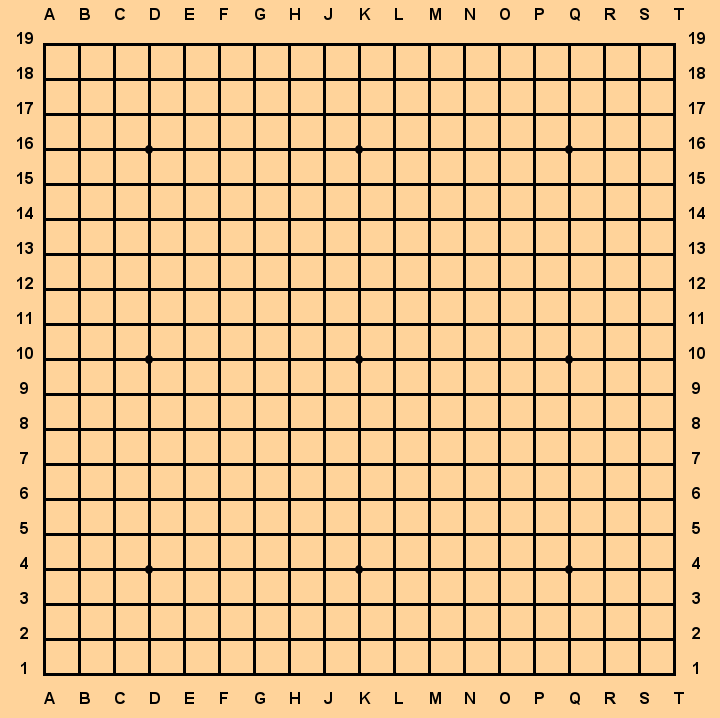
\includegraphics[height=12.25cm]{imgs/goban.png}
          \end{center}
    \item  \textbf{Przechwytywanie kamieni}\\
          Mechanizm przechwytywania kamieni został zrealizowany z wykorzystaniem
          algorytmu flood fill.\\
          Przykłady:\\

          \begin{figure}[H]
              \centering%
              \begin{minipage}{.48\textwidth}%
                  \centering
                  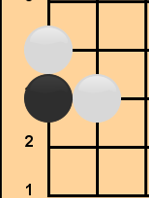
\includegraphics[height=4cm]{imgs/capture1a.png}
                  \centering
                  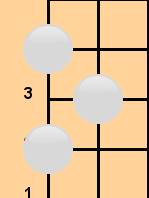
\includegraphics[height=4cm]{imgs/capture1b.png}
              \end{minipage}%
              \captionof{figure}{Białe kamienie otaczają czarny kamień, dlatego czarny kamień zostaje zbity}
          \end{figure}

          \begin{figure}[H]
              \centering%
              \begin{minipage}{.48\textwidth}%
                  \centering
                  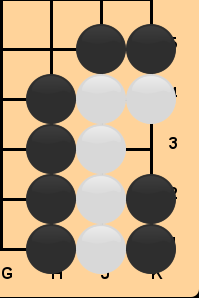
\includegraphics[height=4cm]{imgs/capture2a.png}
                  \centering
                  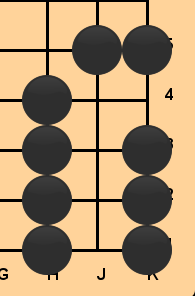
\includegraphics[height=4cm]{imgs/capture2b.png}
              \end{minipage}%
              \captionof{figure}{Czarny kamień przesuwa się na pozycję K3, więc przejmuje
                  kamienie białe}
          \end{figure}
          Więcej przykładów: https://en.wikipedia.org/wiki/Rules\_of\_Go.


          \newpage


    \item  \textbf{Zasada ko} \\
          Jeżeli gracz będzie chciał się zrobić ruch na miejsce, na które ruch
          został wykonany przed chwilą, graczowi ukaże się okienko informujące o
          zasadzie ko. Zasada ko zapobiega powstaniu nieskończonej pętli w grze.

          \begin{figure}[H]
              \centering%
              \begin{minipage}{.48\textwidth}%
                  \centering
                  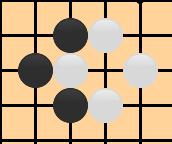
\includegraphics[width=4cm]{imgs/ko_rule1.png}
                  \centering
                  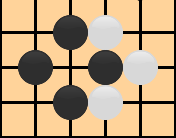
\includegraphics[width=4cm]{imgs/ko_rule2.png}
                  \centering
                  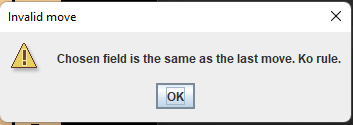
\includegraphics{imgs/ko_rule_warning.png}
                  \centering
              \end{minipage}%
              \captionof{figure}{Jeżeli czarny kamień przechwyci kamień biały,
                  to biały kamień nie może od razu przechwycić kamienia czarnego,
                  tylko musi najpierw wykonać ruch na inne, niezajęte pole, a potem
                  dopiero może przechwycić kamień przeciwnika.}
          \end{figure}
    \item \textbf{Zasada superko}\\
          W grze nie może występować powtórzenie takiego samego ułożenia tablicy. (bardzo
          rzadkie zjawisko), zasada superko sprawdzana jest przy pomocy tablicy
          Zobrista.
          \newpage
    \item \textbf{Samobójstwo}\\
          Zakładam, że nie jest możliwe popełnienie samobójstwa tj. nie można
          ruszyć się na miejsce, które doprowadzi do przejęcia kamienia
          przez przeciwnika. Przy próbie popełnienia samobójstwa użytkownikowi
          ukaże się okienko informujące o zaistniałej sytuacji.

          \begin{figure}[H]
              \centering
              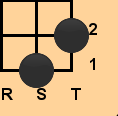
\includegraphics[width=4cm]{imgs/suicide.png}
              \captionof{figure}{Jeżeli czarny kamień wykona ruch na miejsce T1, użytkownikowi
                  ukaże się okienko o błędnym ruchu}
          \end{figure}

          \begin{center}
              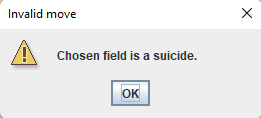
\includegraphics{imgs/suicide_popup.png}
          \end{center}

    \item \textbf{Koniec gry}\\
          Gra kończy się w momencie, w którym nie ma już żadnych ruchów, które
          nie zakończyłyby się samobójstwem, lub jeden z graczy zrezygnuje z gry,
          albo oboje graczy przekażą swój ruch pod rząd.

          \newpage
    \item \textbf{\q{Martwe} kamienie}\\
          Niemożliwa jest implementacja algorytmu znajdująca
          \q{martwe} kamienie, dlatego po zakończeniu gry użytkownikowi
          ukaże się okienko, które umożliwia
          wprowadzenie \q{martwych} kamieni. \q{Martwe} kamienie zdefiniowane
          są jako te, które w późniejszej części gry zostałyby przechwycone przez
          przeciwnika.

          \begin{figure}[H]
            \centering%
            \begin{minipage}{\textwidth}
                \centering
          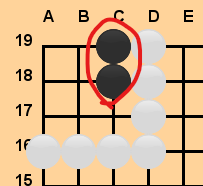
\includegraphics{imgs/deadStones.png}
          \caption{Przykład \q{martwych} kamieni.}
        \end{minipage}
    \end{figure}%


          \newpage
    \item \textbf{Liczenie punktów}\\
          Punkty są liczone, jako miejsca na planszy otoczone wyłącznie
          przez dany kamień. Do oznaczenia punktów także użyłam algorytmu flood fill
          opartym na BFS. Do punktów danego gracza dodawane są punkty
          przechwyconych kamieni przeciwnika i odejmowane są \q{martwe} kamienie.

          %   \begin{center}
          %   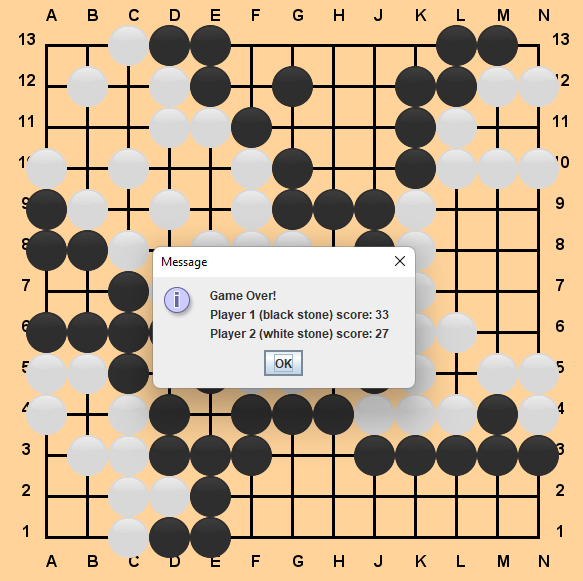
\includegraphics{imgs/gameOver2.png}
          %   \end{center}

          \begin{figure}[H]
              \centering%
              \begin{minipage}{\textwidth}
                  \centering
                  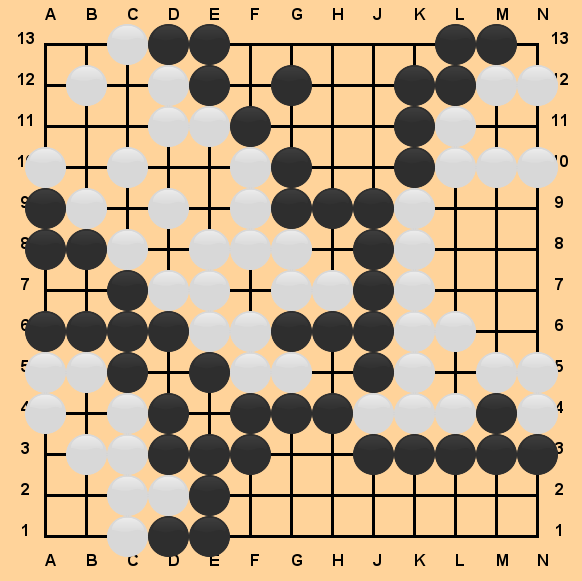
\includegraphics[width=7.5cm]{imgs/countingPointsBoard.png}
                  \caption{Przykład gry (tutaj akurat 13x13)}
                  \centering
                  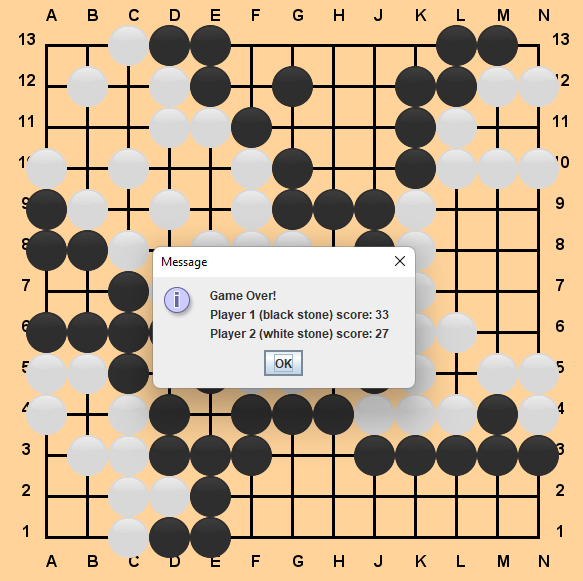
\includegraphics[width=7.5cm]{imgs/gameOver2.png}
                  \caption{Punkty dla poszczególnych graczy policzone przez mój algorytm
                      (bez uwzględnienia \q{martwych} kamieni)}
              \end{minipage}
          \end{figure}%

          \begin{figure}[H]
              \centering%
              \begin{minipage}{\textwidth}
                  \centering
                  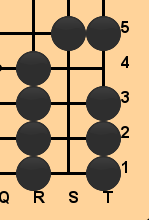
\includegraphics{imgs/countingPoints.png}
              \end{minipage}
              \caption{Przykładowo tutaj wartość punktów dla gracza
                  mającego czarne kamienie będzie równa 5 jeśli gracz nie przechwycił
                  białych kamieni, a jeśli przechwycił 5 kamieni to wartość punktów będzie równa 10}
          \end{figure}% 

    \item \textbf{Zapisywanie stanu gry do plików}\\

          \begin{figure}[H]
              \centering%
              \begin{minipage}{\textwidth}
                  \centering
                  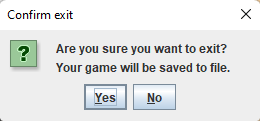
\includegraphics{imgs/confirmExit.png}
              \end{minipage}
              \caption{Przy próbie zamknięcia okna, użytkownik zobaczy okienko potwierdzenia
                  wyjścia z aplikacji. Stan gry będzie automatycznie zapisywany do plików
                  txt (w tym przeszłe ruchy, aktualny ruch gracza i przechwycone kamienie).}
          \end{figure}% 

          \begin{figure}[H]
              \centering%
              \begin{minipage}{\textwidth}
                  \centering
                  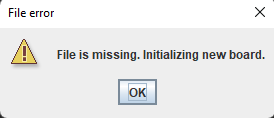
\includegraphics{imgs/missingFile.png}
              \end{minipage}
                \caption{Jeżeli jeden z plików nie istnieje wyświetlana jest taka wiadomość, usuwane są inne pliki i inicjalizowana jest nowa plansza.}
          \end{figure}% 

          %   \begin{center}
          %   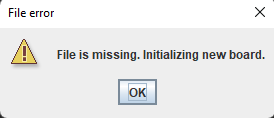
\includegraphics{imgs/missingFile.png}
          %   \end{center}
          %   Jeżeli jeden z plików jest uszkodzony wyświetlana jest taka wiamomość, usuwane są inne pliki i inicjalizowana jest nowa plansza:\\
          \begin{center}
              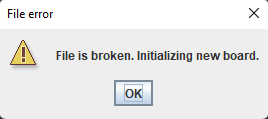
\includegraphics{imgs/brokenFile.png}
          \end{center}
    \item \textbf{Diagram klas UML}\\
          Diagram klas UML zostanie umieszczony w innym pliku, ponieważ jest za duży.\\
    \item \textbf{Źródła}\\
          Zasady gry: https://en.wikipedia.org/wiki/Rules\_of\_Go \\
          Zasady gry: https://www.youtube.com/watch?v=QYNRvMolN20\&t=247s \\
          Zdjęcia kamieni: https://pixabay.com/pl/vectors/czerwony-przycisk-odznaka-okr\%c4\%85g-47690/ \\
          Zobrist Hashing: https://www.geeksforgeeks.org/minimax-algorithm-in-game-theory-set-5-zobrist-hashing/

\end{enumerate} 


\end{document}
